%%%%%%%%%%%%%%%%%%%%%%%%%%%%%%%%%%%%%%%%%%%%%%
%                insertmeeting
% 1) Title (something creative & funny?)
% 2) Date (MM/DD/YYYY)
% 3) Location (ex. Hagerty High School)
% 4) People/Committees Present 
% 5) Picture 
% 6) Start Time & Stop Time (ex. 12:30AM to 4:30PM)
%%%%%%%%%%%%%%%%%%%%%%%%%%%%%%%%%%%%%%%%%%%%%%
\insertmeeting 
	{Vuforia Vision} 
	{01/19/22} 
	{Hagerty High School}
	{Anouska, Falon, James, Nathan, Ritam, Rose, Samantha}
	{Images/RobotPics/robot.jpg}
	{2:30 - 4:30}
	
\hhscommittee{Software}
\noindent\hfil\rule{\textwidth}{.4pt}\hfil
\subsubsection*{Goals}
\begin{itemize}
    \item Setup the Vuforia system to see if it is viable for use in this year's game.  

\end{itemize} 

\noindent\hfil\rule{\textwidth}{.4pt}\hfil

\subsubsection*{Accomplishments}
After fine-tuning the road runner navigation system, we were still running into some issues. For example, the lack of drive encoders on our drivetrain meant that any amount of wheel slippage could greatly throw off our localization. One solution we have brainstormed for this problem is correcting the current estimate of our position using a camera. Because there are Vuforia Vumarks every year, we wanted to explore that approach this time. We used the sample OpMode "ConceptVuforiaFieldNavigationWebcam" to test the method. Standing at the center of the field, the coordinate (0, 0) in code, we pointed the camera at each camera. While the measurements were close to (0, 0), there were fluctuations as we moved the camera further from the target. To adjust for this, we may focus on only enabling Vuforia at close distances to increase the accuracy.


\begin{figure}[htp]
\centering
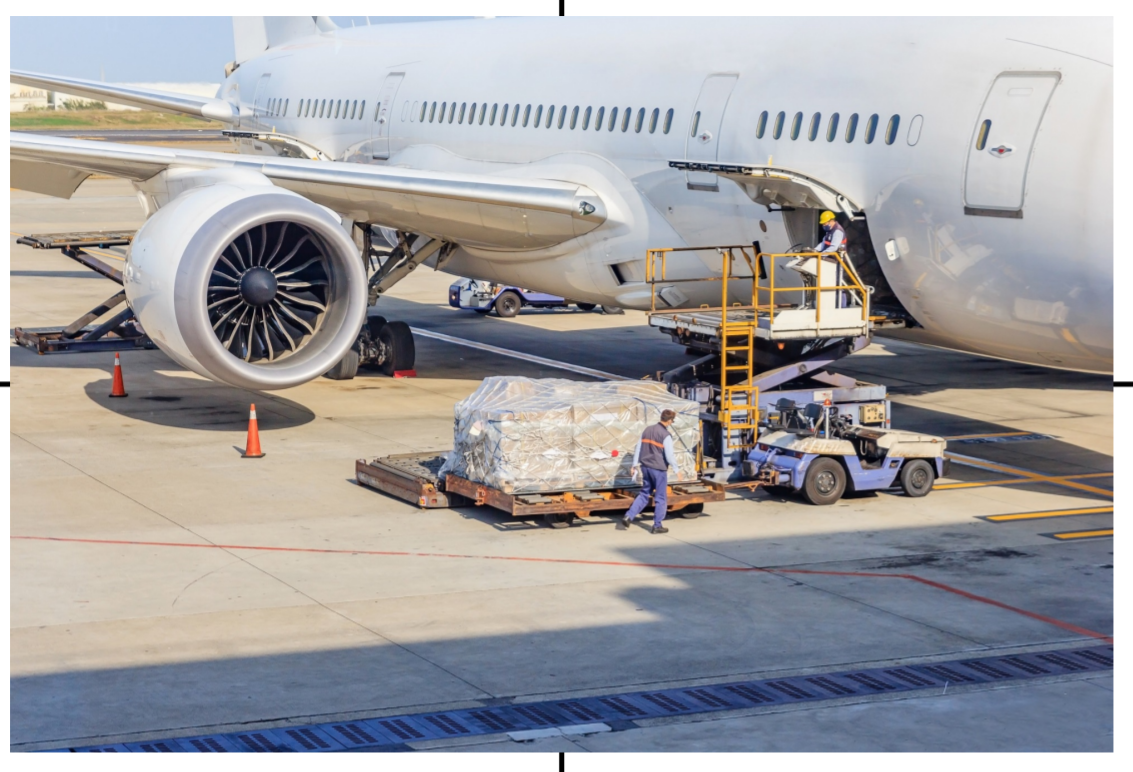
\includegraphics[width=0.95\textwidth, angle=0]{Meetings/January/01-19-22/1.19.21 airplane picture - James Hu.PNG}
\caption{The image with a hidden "VuMark" that we will use Vuforia to detect}
\label{fig:012922_1}
\end{figure}

\whatsnext{
\begin{itemize}
    \item Continue to test Vuforia and find an effective way to integrate it into our current navigational systems.
\end{itemize} 
}

